\SourceLeaf{234}%
\Needspace{10\baselineskip}
\begin{center}[II.]\end{center}
Die Construction für 2 ist:
\[
\begin{aligned}
1&=180^{0}-B\\
2&=180^{0}-C\\
3&=180^{0}-\{180^{0}-(B+C)\}.
\end{aligned}
\]
Man kann aber den Satz 3 mit Einem Schlage durch folgende Construction beweisen:
\begin{center}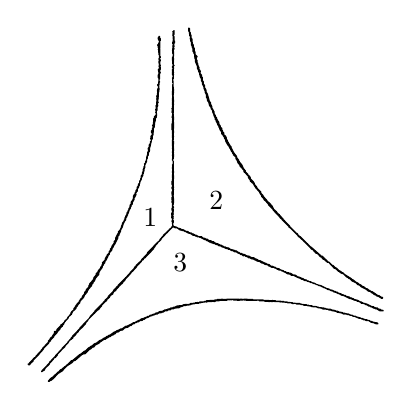
\begin{tikzpicture}[x=0.00514541cm,y=-0.00514541cm]
\fill[even odd rule] (872,739) -- (870,737) -- (868,737) -- (867,736) -- (863,736) -- (862,735) -- (859,735) -- (856,733) -- (853,733) -- (850,731) -- (846,731) -- (844,729) -- (840,729) -- (833,726) -- (830,726) -- (827,724) -- (824,724) -- (823,723) -- (818,722) -- (815,720) -- (811,720) -- (808,718) -- (805,718) -- (799,715) -- (791,714) -- (790,713) -- (786,713) -- (783,711) -- (776,710) -- (772,708) -- (769,708) -- (765,706) -- (758,705) -- (754,703) -- (747,703) -- (746,702) -- (743,702) -- (742,701) -- (739,701) -- (738,700) -- (726,699) -- (725,698) -- (722,698) -- (721,697) -- (718,697) -- (717,696) -- (711,696) -- (707,694) -- (701,694) -- (700,693) -- (696,693) -- (695,692) -- (688,692) -- (687,691) -- (683,691) -- (682,690) -- (679,690) -- (678,689) -- (668,689) -- (667,688) -- (661,688) -- (660,687) -- (648,686) -- (647,685) -- (640,685) -- (639,684) -- (632,684) -- (631,683) -- (619,683) -- (618,682) -- (612,682) -- (611,681) -- (609,682) -- (603,682) -- (602,681) -- (589,681) -- (588,680) -- (563,680) -- (562,679) -- (549,679) -- (548,678) -- (540,678) -- (539,679) -- (537,679) -- (536,678) -- (531,678) -- (530,679) -- (528,678) -- (498,678) -- (497,679) -- (488,679) -- (487,678) -- (485,678) -- (484,679) -- (474,679) -- (473,680) -- (468,680) -- (467,681) -- (456,681) -- (455,682) -- (448,682) -- (445,684) -- (442,684) -- (441,685) -- (431,685) -- (428,687) -- (425,686) -- (424,687) -- (420,687) -- (419,688) -- (415,688) -- (414,689) -- (408,689) -- (405,691) -- (401,691) -- (400,692) -- (398,691) -- (395,691) -- (394,692) -- (391,692) -- (387,694) -- (380,694) -- (379,695) -- (375,695) -- (369,698) -- (366,698) -- (363,700) -- (359,700) -- (356,702) -- (353,702) -- (350,704) -- (344,705) -- (339,708) -- (331,709) -- (327,712) -- (323,712) -- (319,715) -- (314,716) -- (311,718) -- (308,718) -- (305,721) -- (301,721) -- (299,723) -- (297,723) -- (291,726) -- (286,727) -- (281,731) -- (279,731) -- (270,736) -- (267,736) -- (263,739) -- (251,745) -- (248,745) -- (238,752) -- (235,752) -- (230,755) -- (226,756) -- (222,759) -- (220,759) -- (209,767) -- (207,767) -- (203,770) -- (201,770) -- (198,773) -- (193,775) -- (188,779) -- (184,780) -- (175,787) -- (171,788) -- (164,794) -- (161,795) -- (159,797) -- (155,799) -- (148,806) -- (145,807) -- (138,813) -- (134,815) -- (116,830) -- (114,830) -- (112,832) -- (111,832) -- (110,834) -- (98,845) -- (97,845) -- (89,852) -- (86,853) -- (82,858) -- (81,858) -- (67,871) -- (62,874) -- (56,881) -- (56,883) -- (57,884) -- (60,884) -- (62,882) -- (65,881) -- (68,878) -- (69,878) -- (83,863) -- (85,863) -- (88,860) -- (90,860) -- (103,846) -- (117,837) -- (120,833) -- (124,832) -- (140,818) -- (144,816) -- (147,816) -- (149,815) -- (159,805) -- (163,803) -- (167,799) -- (170,799) -- (174,794) -- (182,790) -- (187,785) -- (188,785) -- (195,780) -- (198,780) -- (202,777) -- (205,776) -- (207,774) -- (211,773) -- (214,770) -- (218,769) -- (220,767) -- (223,766) -- (226,762) -- (230,762) -- (235,758) -- (241,757) -- (245,753) -- (249,751) -- (254,750) -- (259,746) -- (262,746) -- (266,742) -- (269,742) -- (272,739) -- (274,739) -- (277,737) -- (280,737) -- (283,734) -- (287,734) -- (288,733) -- (290,733) -- (292,731) -- (294,731) -- (299,727) -- (303,726) -- (310,722) -- (313,722) -- (315,720) -- (318,720) -- (322,718) -- (326,718) -- (330,715) -- (338,714) -- (339,713) -- (341,713) -- (345,710) -- (350,710) -- (354,707) -- (359,707) -- (361,705) -- (366,705) -- (369,703) -- (380,702) -- (385,699) -- (387,699) -- (391,697) -- (396,697) -- (397,696) -- (407,695) -- (411,693) -- (419,692) -- (420,691) -- (429,691) -- (430,690) -- (434,690) -- (435,689) -- (439,689) -- (440,688) -- (444,688) -- (445,687) -- (447,688) -- (449,688) -- (450,687) -- (461,687) -- (462,686) -- (468,687) -- (471,685) -- (479,685) -- (480,684) -- (498,684) -- (500,682) -- (502,682) -- (503,683) -- (505,682) -- (507,682) -- (508,683) -- (510,682) -- (513,682) -- (514,683) -- (523,683) -- (524,684) -- (529,684) -- (530,683) -- (538,683) -- (539,682) -- (541,683) -- (545,683) -- (546,684) -- (572,684) -- (573,683) -- (576,683) -- (578,685) -- (590,685) -- (591,686) -- (600,686) -- (601,687) -- (605,687) -- (606,686) -- (608,687) -- (612,687) -- (613,686) -- (615,686) -- (616,687) -- (628,687) -- (629,688) -- (633,687) -- (634,688) -- (641,688) -- (642,689) -- (647,689) -- (648,690) -- (656,690) -- (660,692) -- (667,691) -- (670,693) -- (679,693) -- (680,694) -- (685,694) -- (688,696) -- (696,696) -- (697,697) -- (705,698) -- (706,699) -- (709,699) -- (710,700) -- (719,700) -- (723,702) -- (731,703) -- (734,705) -- (747,706) -- (750,708) -- (755,708) -- (756,709) -- (767,711) -- (770,713) -- (781,715) -- (787,718) -- (790,717) -- (791,718) -- (794,718) -- (795,719) -- (799,719) -- (803,721) -- (806,721) -- (809,723) -- (812,723) -- (824,728) -- (828,728) -- (831,730) -- (833,730) -- (836,732) -- (839,732) -- (842,734) -- (848,734) -- (854,738) -- (860,739) -- (867,742) -- (871,742) -- (872,741) -- cycle
(332,29) -- (330,29) -- (327,34) -- (327,37) -- (330,43) -- (330,45) -- (328,47) -- (328,49) -- (326,51) -- (326,53) -- (327,54) -- (327,58) -- (328,59) -- (328,61) -- (327,62) -- (328,64) -- (328,70) -- (329,71) -- (329,76) -- (330,77) -- (330,84) -- (329,85) -- (329,88) -- (330,89) -- (329,91) -- (329,97) -- (330,98) -- (329,106) -- (330,107) -- (330,109) -- (327,113) -- (328,115) -- (328,118) -- (329,119) -- (329,122) -- (327,126) -- (327,132) -- (329,135) -- (329,142) -- (328,143) -- (328,147) -- (326,149) -- (326,152) -- (327,153) -- (328,157) -- (326,160) -- (326,163) -- (325,164) -- (326,170) -- (325,171) -- (325,175) -- (323,178) -- (324,180) -- (324,184) -- (323,185) -- (324,187) -- (324,191) -- (323,192) -- (323,200) -- (321,202) -- (322,204) -- (322,209) -- (321,210) -- (321,213) -- (322,214) -- (322,216) -- (321,217) -- (321,219) -- (322,220) -- (322,224) -- (318,228) -- (318,231) -- (316,233) -- (316,242) -- (315,243) -- (315,248) -- (313,250) -- (314,252) -- (314,256) -- (313,257) -- (313,261) -- (310,264) -- (310,267) -- (313,272) -- (309,277) -- (309,281) -- (308,283) -- (310,286) -- (310,288) -- (308,290) -- (308,294) -- (305,298) -- (305,303) -- (302,307) -- (302,309) -- (303,310) -- (303,314) -- (301,316) -- (301,322) -- (300,323) -- (300,326) -- (299,327) -- (298,336) -- (296,339) -- (296,342) -- (293,345) -- (294,349) -- (292,352) -- (292,355) -- (290,359) -- (290,363) -- (288,367) -- (288,371) -- (285,375) -- (285,380) -- (284,381) -- (284,384) -- (281,388) -- (281,392) -- (278,395) -- (278,399) -- (275,403) -- (275,407) -- (272,411) -- (272,414) -- (270,416) -- (270,419) -- (268,421) -- (266,425) -- (266,430) -- (265,431) -- (265,433) -- (260,440) -- (260,444) -- (258,446) -- (258,448) -- (257,449) -- (257,453) -- (255,455) -- (255,458) -- (253,460) -- (253,462) -- (250,466) -- (250,469) -- (247,474) -- (247,476) -- (245,478) -- (245,482) -- (243,484) -- (243,486) -- (239,491) -- (238,496) -- (236,499) -- (236,502) -- (233,508) -- (229,512) -- (229,516) -- (227,518) -- (222,528) -- (222,533) -- (218,537) -- (218,541) -- (213,548) -- (212,552) -- (209,555) -- (209,558) -- (206,562) -- (206,565) -- (201,570) -- (201,572) -- (199,574) -- (196,580) -- (196,582) -- (189,589) -- (190,592) -- (188,595) -- (188,597) -- (185,600) -- (185,602) -- (179,609) -- (178,612) -- (174,616) -- (174,619) -- (168,626) -- (168,628) -- (166,632) -- (158,641) -- (158,643) -- (156,645) -- (156,648) -- (155,650) -- (150,655) -- (149,658) -- (146,661) -- (145,666) -- (140,672) -- (139,676) -- (135,679) -- (134,682) -- (132,684) -- (132,686) -- (127,690) -- (127,691) -- (123,696) -- (122,699) -- (119,702) -- (119,705) -- (117,707) -- (116,707) -- (112,712) -- (111,716) -- (104,724) -- (103,727) -- (97,732) -- (96,735) -- (91,740) -- (87,742) -- (87,744) -- (77,754) -- (77,756) -- (75,758) -- (72,758) -- (71,759) -- (71,762) -- (69,766) -- (67,768) -- (66,771) -- (60,776) -- (60,778) -- (56,782) -- (56,785) -- (42,800) -- (42,801) -- (38,805) -- (38,806) -- (25,820) -- (25,821) -- (23,823) -- (22,823) -- (7,839) -- (6,839) -- (6,841) -- (8,843) -- (11,843) -- (13,841) -- (13,840) -- (21,833) -- (21,831) -- (35,817) -- (35,816) -- (45,805) -- (47,801) -- (59,789) -- (60,786) -- (64,783) -- (64,781) -- (72,773) -- (72,771) -- (79,764) -- (81,760) -- (87,754) -- (88,751) -- (93,747) -- (93,745) -- (96,742) -- (98,737) -- (108,726) -- (108,724) -- (115,718) -- (118,711) -- (121,708) -- (122,708) -- (127,702) -- (127,700) -- (130,697) -- (132,693) -- (136,689) -- (136,686) -- (146,675) -- (147,671) -- (154,663) -- (155,659) -- (157,657) -- (157,656) -- (165,647) -- (166,643) -- (169,640) -- (169,638) -- (172,635) -- (175,628) -- (183,619) -- (183,615) -- (186,609) -- (190,604) -- (192,600) -- (192,598) -- (194,596) -- (195,593) -- (198,590) -- (198,587) -- (202,582) -- (202,580) -- (204,578) -- (206,572) -- (209,569) -- (209,566) -- (215,559) -- (216,554) -- (218,552) -- (220,547) -- (222,545) -- (230,529) -- (230,525) -- (233,522) -- (233,520) -- (237,512) -- (237,509) -- (241,502) -- (243,495) -- (247,487) -- (249,485) -- (250,479) -- (252,477) -- (252,475) -- (254,472) -- (254,470) -- (256,467) -- (258,460) -- (261,455) -- (261,453) -- (263,451) -- (263,448) -- (266,445) -- (266,441) -- (270,434) -- (270,430) -- (272,428) -- (275,421) -- (274,418) -- (278,413) -- (278,408) -- (281,404) -- (281,402) -- (283,399) -- (283,395) -- (284,394) -- (285,389) -- (288,384) -- (288,381) -- (292,374) -- (292,371) -- (293,370) -- (293,367) -- (294,366) -- (294,363) -- (295,362) -- (295,358) -- (297,354) -- (297,348) -- (301,340) -- (301,335) -- (303,332) -- (303,327) -- (305,325) -- (306,317) -- (308,315) -- (309,303) -- (310,302) -- (310,299) -- (311,298) -- (311,295) -- (312,294) -- (313,286) -- (315,284) -- (315,277) -- (317,274) -- (318,258) -- (320,255) -- (320,250) -- (321,249) -- (321,243) -- (322,242) -- (323,233) -- (325,231) -- (325,228) -- (326,227) -- (325,216) -- (327,213) -- (327,205) -- (329,202) -- (328,200) -- (328,196) -- (330,194) -- (329,192) -- (329,186) -- (330,185) -- (329,182) -- (330,181) -- (330,169) -- (331,168) -- (331,164) -- (332,163) -- (331,151) -- (332,150) -- (332,145) -- (333,144) -- (333,142) -- (332,141) -- (332,137) -- (333,136) -- (333,124) -- (335,120) -- (334,118) -- (334,113) -- (335,112) -- (335,106) -- (334,105) -- (335,103) -- (335,101) -- (334,100) -- (334,92) -- (335,91) -- (335,88) -- (333,86) -- (333,85) -- (335,83) -- (335,80) -- (334,79) -- (334,62) -- (333,61) -- (334,59) -- (334,46) -- (333,44) -- (335,41) -- (335,36) -- (333,33) -- (333,30) -- cycle
(368,15) -- (367,15) -- (363,19) -- (364,21) -- (363,28) -- (364,29) -- (364,36) -- (365,38) -- (364,39) -- (364,43) -- (363,44) -- (363,49) -- (364,50) -- (363,57) -- (364,59) -- (363,60) -- (363,64) -- (362,65) -- (363,67) -- (363,73) -- (364,74) -- (364,79) -- (362,83) -- (363,99) -- (364,100) -- (364,102) -- (362,105) -- (362,107) -- (364,109) -- (364,110) -- (362,112) -- (362,115) -- (363,116) -- (362,118) -- (362,125) -- (363,126) -- (364,130) -- (362,134) -- (363,135) -- (363,145) -- (364,146) -- (364,148) -- (363,149) -- (363,165) -- (362,166) -- (362,175) -- (363,176) -- (363,182) -- (362,183) -- (362,191) -- (363,192) -- (362,194) -- (362,200) -- (363,202) -- (362,204) -- (363,206) -- (361,208) -- (361,210) -- (362,211) -- (361,218) -- (363,221) -- (363,223) -- (362,224) -- (362,228) -- (361,230) -- (363,233) -- (362,235) -- (363,238) -- (362,239) -- (362,245) -- (361,246) -- (361,261) -- (362,262) -- (362,272) -- (363,273) -- (362,275) -- (362,281) -- (363,282) -- (363,285) -- (362,286) -- (362,302) -- (363,303) -- (363,305) -- (362,306) -- (362,308) -- (363,309) -- (363,314) -- (362,315) -- (362,318) -- (363,319) -- (363,322) -- (362,323) -- (362,325) -- (363,326) -- (363,332) -- (362,333) -- (362,336) -- (364,339) -- (364,345) -- (362,348) -- (363,350) -- (363,352) -- (362,353) -- (362,357) -- (363,358) -- (363,362) -- (362,363) -- (362,367) -- (363,368) -- (363,371) -- (362,372) -- (362,379) -- (363,381) -- (362,382) -- (362,387) -- (361,388) -- (361,396) -- (363,400) -- (361,403) -- (361,406) -- (362,407) -- (362,410) -- (363,412) -- (361,414) -- (361,419) -- (362,420) -- (361,422) -- (362,424) -- (362,427) -- (361,428) -- (361,435) -- (362,436) -- (361,438) -- (361,441) -- (362,442) -- (362,454) -- (361,455) -- (361,460) -- (362,461) -- (362,464) -- (360,468) -- (360,472) -- (361,473) -- (360,478) -- (362,481) -- (362,485) -- (361,486) -- (361,488) -- (362,489) -- (362,494) -- (363,495) -- (363,498) -- (361,500) -- (361,501) -- (357,505) -- (356,505) -- (354,507) -- (354,508) -- (340,521) -- (340,522) -- (332,531) -- (330,535) -- (328,537) -- (327,537) -- (301,564) -- (300,567) -- (292,575) -- (292,576) -- (288,579) -- (285,584) -- (273,595) -- (273,596) -- (269,600) -- (267,604) -- (258,613) -- (258,614) -- (251,621) -- (251,622) -- (248,625) -- (247,625) -- (246,627) -- (228,645) -- (228,646) -- (224,649) -- (224,650) -- (217,657) -- (216,660) -- (204,672) -- (203,675) -- (196,681) -- (196,682) -- (192,686) -- (192,687) -- (171,708) -- (171,709) -- (167,713) -- (167,714) -- (160,721) -- (157,726) -- (142,741) -- (142,742) -- (134,750) -- (134,751) -- (128,757) -- (128,758) -- (116,770) -- (116,771) -- (112,775) -- (112,776) -- (104,785) -- (104,786) -- (90,800) -- (90,801) -- (82,809) -- (82,810) -- (74,818) -- (74,819) -- (64,829) -- (64,830) -- (60,833) -- (58,837) -- (39,857) -- (39,859) -- (40,860) -- (42,860) -- (44,858) -- (48,856) -- (51,850) -- (60,842) -- (61,839) -- (67,833) -- (67,832) -- (71,828) -- (71,827) -- (73,825) -- (75,825) -- (77,823) -- (77,822) -- (80,819) -- (81,816) -- (90,807) -- (90,806) -- (99,798) -- (100,795) -- (107,788) -- (109,784) -- (113,780) -- (114,780) -- (119,776) -- (119,774) -- (121,772) -- (122,772) -- (127,766) -- (127,765) -- (132,761) -- (133,758) -- (144,748) -- (144,747) -- (150,741) -- (151,738) -- (156,733) -- (156,731) -- (171,716) -- (172,716) -- (173,714) -- (180,707) -- (181,707) -- (185,703) -- (185,702) -- (190,697) -- (190,695) -- (199,686) -- (200,686) -- (202,684) -- (203,681) -- (209,676) -- (210,673) -- (213,670) -- (217,668) -- (219,663) -- (221,661) -- (225,659) -- (225,657) -- (232,650) -- (232,649) -- (242,640) -- (242,639) -- (247,634) -- (249,630) -- (257,622) -- (257,621) -- (262,616) -- (262,615) -- (269,609) -- (269,608) -- (275,602) -- (278,597) -- (282,594) -- (282,593) -- (288,587) -- (288,586) -- (290,584) -- (291,584) -- (293,582) -- (293,581) -- (295,579) -- (296,579) -- (318,556) -- (319,553) -- (321,551) -- (323,547) -- (328,542) -- (328,541) -- (337,533) -- (337,531) -- (346,522) -- (346,521) -- (350,517) -- (351,517) -- (353,515) -- (353,514) -- (365,502) -- (371,505) -- (375,505) -- (382,510) -- (385,510) -- (386,511) -- (392,512) -- (394,514) -- (396,514) -- (401,517) -- (408,519) -- (414,523) -- (418,523) -- (420,525) -- (422,525) -- (425,527) -- (429,527) -- (430,528) -- (432,528) -- (443,534) -- (445,534) -- (449,537) -- (451,537) -- (455,540) -- (457,540) -- (459,542) -- (462,542) -- (463,543) -- (468,544) -- (471,546) -- (474,546) -- (478,549) -- (482,549) -- (486,552) -- (488,552) -- (496,556) -- (499,556) -- (502,558) -- (505,558) -- (509,561) -- (512,561) -- (517,564) -- (521,564) -- (525,567) -- (529,568) -- (532,571) -- (535,571) -- (538,574) -- (542,573) -- (544,575) -- (548,576) -- (552,579) -- (555,579) -- (558,581) -- (564,582) -- (566,584) -- (568,584) -- (573,587) -- (579,588) -- (581,590) -- (585,592) -- (587,592) -- (592,595) -- (598,596) -- (601,599) -- (603,599) -- (608,602) -- (613,602) -- (616,604) -- (618,604) -- (622,607) -- (624,607) -- (626,609) -- (631,609) -- (633,611) -- (637,612) -- (639,614) -- (641,614) -- (647,618) -- (653,619) -- (657,622) -- (662,622) -- (674,628) -- (676,628) -- (683,632) -- (685,632) -- (690,635) -- (694,635) -- (697,637) -- (702,638) -- (705,640) -- (708,640) -- (711,642) -- (716,643) -- (718,645) -- (721,645) -- (724,647) -- (729,648) -- (731,650) -- (733,650) -- (738,653) -- (740,653) -- (747,657) -- (752,658) -- (755,660) -- (758,660) -- (762,663) -- (767,664) -- (772,667) -- (774,667) -- (781,671) -- (786,672) -- (800,679) -- (806,680) -- (807,681) -- (809,681) -- (811,683) -- (817,684) -- (820,686) -- (825,687) -- (830,691) -- (834,691) -- (835,692) -- (837,692) -- (842,695) -- (844,695) -- (848,698) -- (851,698) -- (853,700) -- (855,700) -- (860,703) -- (862,703) -- (865,705) -- (868,705) -- (876,710) -- (884,710) -- (885,709) -- (885,707) -- (884,706) -- (879,705) -- (877,703) -- (873,703) -- (870,700) -- (866,700) -- (865,699) -- (863,699) -- (861,697) -- (855,696) -- (843,690) -- (841,690) -- (840,689) -- (835,688) -- (830,685) -- (828,685) -- (821,681) -- (813,679) -- (811,677) -- (809,677) -- (806,675) -- (803,675) -- (801,673) -- (793,671) -- (791,669) -- (788,669) -- (785,667) -- (783,667) -- (780,665) -- (773,663) -- (771,661) -- (769,661) -- (766,659) -- (764,659) -- (758,656) -- (753,655) -- (750,653) -- (745,652) -- (731,645) -- (720,642) -- (713,638) -- (710,638) -- (705,635) -- (702,635) -- (699,633) -- (697,633) -- (695,631) -- (690,630) -- (686,627) -- (684,627) -- (678,624) -- (673,623) -- (668,619) -- (661,618) -- (659,616) -- (655,614) -- (652,614) -- (651,613) -- (645,612) -- (643,610) -- (640,610) -- (638,608) -- (631,606) -- (627,603) -- (621,602) -- (617,599) -- (615,599) -- (611,597) -- (607,597) -- (603,593) -- (598,592) -- (594,589) -- (592,589) -- (580,583) -- (577,583) -- (573,580) -- (567,578) -- (565,576) -- (560,576) -- (553,572) -- (547,571) -- (542,568) -- (537,567) -- (534,565) -- (531,565) -- (529,563) -- (527,563) -- (522,559) -- (519,559) -- (518,558) -- (507,555) -- (503,552) -- (497,551) -- (494,549) -- (491,549) -- (489,547) -- (487,547) -- (485,545) -- (483,545) -- (475,541) -- (470,540) -- (465,536) -- (462,536) -- (459,534) -- (456,534) -- (452,532) -- (450,530) -- (447,530) -- (444,528) -- (439,527) -- (436,524) -- (429,524) -- (422,520) -- (420,520) -- (415,517) -- (413,517) -- (411,515) -- (405,514) -- (402,511) -- (398,511) -- (391,507) -- (386,506) -- (383,504) -- (378,503) -- (373,500) -- (368,499) -- (366,497) -- (366,491) -- (367,490) -- (367,485) -- (366,484) -- (366,481) -- (367,480) -- (366,478) -- (367,476) -- (366,474) -- (366,472) -- (367,471) -- (366,469) -- (367,467) -- (366,465) -- (367,463) -- (367,457) -- (366,455) -- (368,453) -- (366,449) -- (366,447) -- (367,446) -- (367,442) -- (368,441) -- (368,431) -- (367,430) -- (367,426) -- (366,425) -- (367,423) -- (367,410) -- (368,409) -- (367,407) -- (367,405) -- (368,404) -- (368,402) -- (367,401) -- (367,383) -- (368,382) -- (367,368) -- (368,367) -- (368,364) -- (367,363) -- (367,339) -- (366,338) -- (366,334) -- (367,333) -- (367,329) -- (368,328) -- (368,322) -- (367,321) -- (367,319) -- (368,318) -- (367,316) -- (367,314) -- (368,313) -- (368,308) -- (367,307) -- (367,305) -- (368,304) -- (367,302) -- (368,290) -- (366,288) -- (367,286) -- (367,279) -- (368,278) -- (367,276) -- (367,269) -- (368,268) -- (368,264) -- (367,263) -- (367,259) -- (368,258) -- (368,242) -- (367,241) -- (367,238) -- (368,237) -- (368,229) -- (367,228) -- (367,223) -- (366,222) -- (367,220) -- (367,200) -- (368,199) -- (368,197) -- (367,196) -- (367,194) -- (368,193) -- (368,187) -- (367,186) -- (367,179) -- (366,177) -- (367,176) -- (367,171) -- (368,170) -- (368,167) -- (367,166) -- (368,164) -- (368,161) -- (367,160) -- (366,136) -- (367,135) -- (367,126) -- (368,125) -- (367,123) -- (367,121) -- (368,120) -- (367,118) -- (367,111) -- (368,110) -- (367,105) -- (369,103) -- (369,102) -- (367,100) -- (367,95) -- (368,94) -- (367,92) -- (367,90) -- (368,89) -- (368,85) -- (367,84) -- (367,80) -- (368,79) -- (368,68) -- (367,67) -- (367,65) -- (369,61) -- (368,59) -- (368,57) -- (369,56) -- (368,49) -- (370,47) -- (370,42) -- (369,41) -- (369,31) -- (368,30) -- (368,27) -- (369,26) -- (369,16) -- cycle
(403,9) -- (402,10) -- (402,17) -- (404,20) -- (405,29) -- (407,32) -- (406,37) -- (407,38) -- (407,42) -- (409,45) -- (409,52) -- (411,55) -- (411,57) -- (413,61) -- (413,68) -- (415,71) -- (415,73) -- (417,75) -- (417,82) -- (418,83) -- (418,86) -- (419,87) -- (419,93) -- (424,105) -- (424,110) -- (427,116) -- (427,118) -- (429,121) -- (430,127) -- (431,128) -- (431,131) -- (434,136) -- (434,140) -- (436,144) -- (436,148) -- (440,156) -- (440,159) -- (443,166) -- (443,169) -- (446,175) -- (446,181) -- (448,184) -- (449,190) -- (452,194) -- (454,202) -- (458,207) -- (458,210) -- (461,213) -- (462,219) -- (464,222) -- (465,227) -- (468,233) -- (468,236) -- (470,238) -- (470,240) -- (474,247) -- (474,249) -- (477,253) -- (477,255) -- (479,258) -- (480,262) -- (484,267) -- (484,271) -- (485,273) -- (488,276) -- (488,277) -- (490,279) -- (491,283) -- (493,285) -- (494,290) -- (496,294) -- (498,296) -- (498,298) -- (501,301) -- (504,307) -- (506,309) -- (506,311) -- (508,313) -- (508,315) -- (511,318) -- (511,320) -- (513,322) -- (513,324) -- (519,329) -- (519,333) -- (522,337) -- (524,343) -- (529,349) -- (529,351) -- (539,362) -- (539,365) -- (540,367) -- (542,368) -- (550,377) -- (550,380) -- (555,387) -- (555,389) -- (562,395) -- (568,405) -- (577,415) -- (580,421) -- (582,423) -- (583,427) -- (588,432) -- (588,434) -- (595,440) -- (595,441) -- (599,445) -- (600,448) -- (611,459) -- (611,460) -- (628,478) -- (628,479) -- (633,483) -- (633,484) -- (650,501) -- (650,502) -- (652,504) -- (653,504) -- (673,524) -- (673,525) -- (675,527) -- (676,527) -- (682,533) -- (683,533) -- (687,537) -- (687,538) -- (689,539) -- (704,554) -- (704,555) -- (706,557) -- (709,558) -- (717,567) -- (721,568) -- (725,572) -- (725,573) -- (730,577) -- (731,577) -- (735,582) -- (738,583) -- (746,590) -- (749,590) -- (762,604) -- (767,606) -- (773,612) -- (774,612) -- (779,616) -- (783,618) -- (785,618) -- (793,626) -- (796,627) -- (799,630) -- (801,630) -- (807,636) -- (816,640) -- (821,645) -- (825,646) -- (829,650) -- (841,656) -- (847,661) -- (852,662) -- (855,665) -- (858,666) -- (861,669) -- (866,671) -- (868,673) -- (872,674) -- (880,679) -- (882,679) -- (884,677) -- (884,675) -- (883,674) -- (879,673) -- (875,670) -- (871,669) -- (858,660) -- (854,659) -- (852,657) -- (849,656) -- (846,653) -- (842,652) -- (837,648) -- (832,646) -- (829,643) -- (826,642) -- (823,639) -- (817,636) -- (811,631) -- (808,630) -- (805,627) -- (789,617) -- (785,613) -- (782,612) -- (780,610) -- (776,608) -- (770,602) -- (766,600) -- (761,595) -- (759,595) -- (751,587) -- (748,586) -- (746,584) -- (746,583) -- (744,581) -- (743,581) -- (734,572) -- (732,572) -- (707,550) -- (706,550) -- (699,543) -- (698,541) -- (697,541) -- (680,524) -- (679,524) -- (674,519) -- (674,518) -- (672,516) -- (671,516) -- (654,499) -- (654,498) -- (642,486) -- (642,485) -- (638,482) -- (638,481) -- (633,476) -- (633,475) -- (629,471) -- (629,470) -- (627,469) -- (622,464) -- (622,463) -- (615,457) -- (611,449) -- (607,445) -- (607,444) -- (598,436) -- (598,435) -- (590,426) -- (588,422) -- (583,417) -- (583,414) -- (574,405) -- (573,402) -- (567,395) -- (567,393) -- (564,388) -- (557,381) -- (557,379) -- (555,375) -- (551,372) -- (551,370) -- (545,364) -- (545,362) -- (540,356) -- (536,347) -- (530,340) -- (530,339) -- (528,337) -- (528,335) -- (524,330) -- (523,326) -- (516,317) -- (510,305) -- (510,303) -- (506,299) -- (506,297) -- (503,294) -- (503,292) -- (501,290) -- (500,286) -- (498,284) -- (498,280) -- (497,279) -- (497,277) -- (492,273) -- (492,269) -- (489,266) -- (489,264) -- (487,261) -- (487,257) -- (483,254) -- (483,251) -- (480,247) -- (479,241) -- (477,239) -- (474,233) -- (474,231) -- (471,228) -- (471,226) -- (468,221) -- (468,217) -- (462,206) -- (462,203) -- (459,197) -- (459,194) -- (456,190) -- (451,172) -- (448,167) -- (448,163) -- (444,156) -- (444,151) -- (441,147) -- (441,142) -- (439,139) -- (439,132) -- (437,130) -- (437,126) -- (433,121) -- (434,117) -- (433,116) -- (433,114) -- (430,111) -- (431,108) -- (428,102) -- (427,96) -- (426,95) -- (426,90) -- (424,87) -- (424,84) -- (426,80) -- (421,75) -- (421,70) -- (419,66) -- (419,60) -- (417,57) -- (416,50) -- (414,48) -- (413,36) -- (411,34) -- (411,28) -- (409,24) -- (409,21) -- (407,19) -- (407,11) -- (405,9) -- cycle;
\node[inner sep=0pt] at (309,477) {$1$};
\node[inner sep=0pt] at (472,435) {$2$};
\node[inner sep=0pt] at (383,589) {$3$};
\end{tikzpicture}
\hspace{.5em}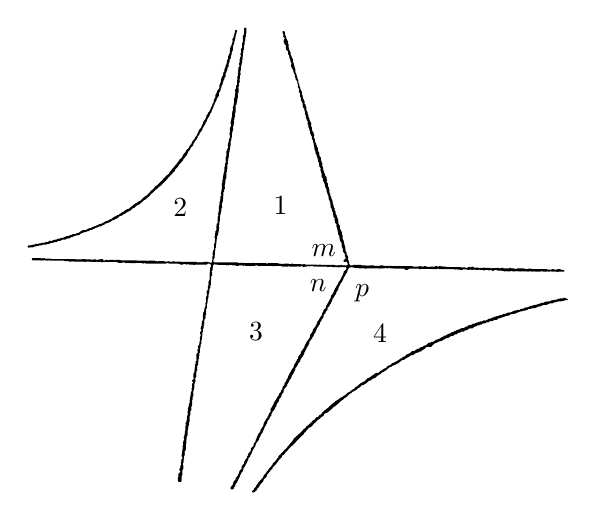
\begin{tikzpicture}[x=0.00536398cm,y=-0.00536398cm]
\fill[even odd rule] (1286,652) -- (1282,652) -- (1280,650) -- (1275,650) -- (1274,651) -- (1266,651) -- (1265,652) -- (1262,652) -- (1259,654) -- (1246,656) -- (1243,658) -- (1232,659) -- (1226,662) -- (1222,662) -- (1218,664) -- (1215,664) -- (1212,666) -- (1204,667) -- (1203,668) -- (1197,669) -- (1191,672) -- (1184,673) -- (1178,676) -- (1174,676) -- (1172,678) -- (1167,678) -- (1166,679) -- (1159,680) -- (1151,684) -- (1143,685) -- (1137,688) -- (1132,688) -- (1130,690) -- (1127,690) -- (1126,691) -- (1123,691) -- (1120,693) -- (1117,693) -- (1113,695) -- (1110,695) -- (1107,697) -- (1105,697) -- (1103,699) -- (1099,699) -- (1091,704) -- (1089,703) -- (1086,703) -- (1084,705) -- (1077,706) -- (1076,707) -- (1068,709) -- (1065,711) -- (1061,711) -- (1059,713) -- (1050,715) -- (1047,718) -- (1044,718) -- (1040,721) -- (1032,722) -- (1030,724) -- (1023,726) -- (1021,728) -- (1018,728) -- (1016,730) -- (1009,732) -- (1005,735) -- (1002,735) -- (1000,737) -- (996,739) -- (993,739) -- (989,743) -- (987,743) -- (983,746) -- (981,746) -- (979,748) -- (973,749) -- (970,752) -- (966,754) -- (963,754) -- (960,756) -- (956,756) -- (951,761) -- (947,763) -- (945,763) -- (942,766) -- (939,766) -- (935,768) -- (933,770) -- (929,771) -- (921,776) -- (917,776) -- (910,782) -- (908,782) -- (904,784) -- (899,789) -- (896,789) -- (892,793) -- (890,793) -- (884,798) -- (882,798) -- (880,800) -- (872,804) -- (870,804) -- (865,809) -- (861,810) -- (859,812) -- (858,812) -- (855,816) -- (851,817) -- (846,821) -- (843,822) -- (839,826) -- (837,827) -- (833,827) -- (829,829) -- (826,832) -- (823,833) -- (817,838) -- (812,840) -- (805,847) -- (795,852) -- (787,859) -- (784,860) -- (780,865) -- (777,866) -- (768,873) -- (765,874) -- (759,880) -- (756,881) -- (751,885) -- (749,885) -- (743,890) -- (736,894) -- (731,899) -- (730,899) -- (726,903) -- (725,903) -- (717,911) -- (716,911) -- (712,915) -- (711,915) -- (703,923) -- (703,924) -- (701,926) -- (699,926) -- (694,932) -- (691,932) -- (686,938) -- (682,940) -- (681,942) -- (675,948) -- (674,948) -- (670,952) -- (669,952) -- (666,955) -- (666,956) -- (663,959) -- (662,959) -- (651,971) -- (648,972) -- (647,974) -- (638,982) -- (633,990) -- (627,996) -- (627,997) -- (622,1002) -- (622,1003) -- (617,1008) -- (616,1008) -- (615,1010) -- (606,1019) -- (606,1020) -- (601,1024) -- (601,1027) -- (597,1030) -- (597,1032) -- (594,1035) -- (594,1036) -- (587,1042) -- (587,1044) -- (585,1046) -- (585,1047) -- (579,1053) -- (577,1057) -- (573,1061) -- (572,1064) -- (566,1070) -- (565,1074) -- (553,1087) -- (552,1090) -- (549,1093) -- (548,1096) -- (543,1101) -- (543,1103) -- (539,1107) -- (539,1109) -- (540,1110) -- (543,1110) -- (549,1105) -- (552,1100) -- (556,1096) -- (556,1094) -- (558,1092) -- (558,1091) -- (564,1085) -- (567,1078) -- (571,1075) -- (574,1070) -- (574,1068) -- (581,1060) -- (581,1059) -- (587,1053) -- (587,1051) -- (596,1042) -- (596,1041) -- (600,1037) -- (602,1033) -- (609,1026) -- (609,1024) -- (611,1022) -- (612,1022) -- (616,1018) -- (616,1017) -- (622,1011) -- (624,1010) -- (624,1008) -- (632,1000) -- (633,1000) -- (657,975) -- (658,975) -- (660,973) -- (662,969) -- (666,966) -- (666,965) -- (673,957) -- (677,956) -- (683,950) -- (683,949) -- (691,942) -- (691,941) -- (693,939) -- (697,937) -- (703,931) -- (705,931) -- (709,927) -- (709,925) -- (711,923) -- (717,921) -- (721,917) -- (722,917) -- (726,913) -- (727,913) -- (732,907) -- (734,907) -- (752,891) -- (753,891) -- (757,887) -- (761,885) -- (769,877) -- (772,876) -- (776,872) -- (779,871) -- (781,869) -- (783,869) -- (791,862) -- (793,862) -- (797,857) -- (801,856) -- (807,853) -- (815,846) -- (819,845) -- (824,841) -- (830,839) -- (835,834) -- (842,830) -- (846,826) -- (849,825) -- (851,823) -- (853,823) -- (865,813) -- (868,813) -- (871,810) -- (873,810) -- (885,804) -- (893,797) -- (896,797) -- (900,795) -- (902,793) -- (910,789) -- (913,786) -- (920,785) -- (926,780) -- (932,779) -- (934,777) -- (937,777) -- (943,772) -- (945,772) -- (951,766) -- (961,766) -- (963,765) -- (965,763) -- (965,762) -- (971,757) -- (973,757) -- (976,755) -- (978,755) -- (981,753) -- (988,751) -- (998,745) -- (1001,745) -- (1005,743) -- (1007,741) -- (1009,741) -- (1010,740) -- (1014,740) -- (1017,737) -- (1019,736) -- (1022,736) -- (1024,734) -- (1028,732) -- (1030,732) -- (1033,730) -- (1039,730) -- (1042,727) -- (1045,727) -- (1053,722) -- (1060,722) -- (1063,719) -- (1067,717) -- (1069,717) -- (1071,715) -- (1075,715) -- (1078,713) -- (1081,713) -- (1085,710) -- (1090,710) -- (1092,708) -- (1097,708) -- (1101,705) -- (1107,705) -- (1111,702) -- (1117,702) -- (1119,700) -- (1123,698) -- (1127,698) -- (1129,696) -- (1135,695) -- (1137,693) -- (1144,692) -- (1145,691) -- (1147,691) -- (1149,689) -- (1152,689) -- (1153,688) -- (1162,687) -- (1164,685) -- (1166,685) -- (1173,682) -- (1176,682) -- (1180,680) -- (1185,680) -- (1187,678) -- (1190,678) -- (1192,676) -- (1197,676) -- (1198,675) -- (1204,675) -- (1205,674) -- (1208,674) -- (1217,670) -- (1221,670) -- (1223,668) -- (1225,668) -- (1226,667) -- (1237,666) -- (1239,664) -- (1241,664) -- (1242,663) -- (1249,663) -- (1252,661) -- (1258,660) -- (1259,659) -- (1262,659) -- (1263,658) -- (1271,658) -- (1272,657) -- (1276,657) -- (1279,655) -- (1284,655) -- (1286,653) -- cycle
(501,16) -- (500,16) -- (498,18) -- (498,23) -- (497,24) -- (497,27) -- (495,31) -- (495,34) -- (492,38) -- (493,43) -- (492,44) -- (492,47) -- (491,48) -- (490,53) -- (488,55) -- (488,58) -- (487,59) -- (487,64) -- (486,65) -- (486,71) -- (484,74) -- (484,76) -- (482,78) -- (482,85) -- (480,87) -- (478,98) -- (476,100) -- (476,103) -- (473,110) -- (473,114) -- (471,116) -- (470,124) -- (467,127) -- (467,129) -- (466,130) -- (466,133) -- (465,134) -- (465,140) -- (463,142) -- (463,145) -- (461,147) -- (461,154) -- (456,161) -- (455,165) -- (452,170) -- (452,176) -- (450,178) -- (450,180) -- (448,182) -- (448,186) -- (447,187) -- (447,189) -- (445,191) -- (445,194) -- (442,199) -- (442,201) -- (439,205) -- (438,209) -- (434,213) -- (434,215) -- (431,218) -- (430,224) -- (428,226) -- (428,228) -- (423,234) -- (423,238) -- (420,241) -- (420,244) -- (418,246) -- (418,248) -- (414,252) -- (407,267) -- (405,269) -- (402,275) -- (398,279) -- (395,286) -- (392,289) -- (389,295) -- (382,302) -- (382,304) -- (376,311) -- (374,315) -- (374,317) -- (367,323) -- (366,326) -- (362,330) -- (362,331) -- (355,339) -- (355,340) -- (349,346) -- (349,347) -- (345,351) -- (342,356) -- (339,359) -- (338,359) -- (314,384) -- (310,386) -- (308,388) -- (308,389) -- (301,396) -- (300,396) -- (298,398) -- (298,399) -- (289,408) -- (284,411) -- (275,420) -- (270,422) -- (268,424) -- (262,427) -- (246,440) -- (243,440) -- (241,442) -- (238,443) -- (235,446) -- (232,447) -- (230,449) -- (226,451) -- (223,454) -- (220,454) -- (218,456) -- (211,459) -- (207,463) -- (205,463) -- (197,468) -- (194,468) -- (184,474) -- (176,476) -- (174,478) -- (172,478) -- (169,480) -- (166,480) -- (164,482) -- (162,482) -- (157,485) -- (151,486) -- (147,489) -- (144,489) -- (143,490) -- (138,490) -- (134,492) -- (129,496) -- (127,496) -- (120,499) -- (115,499) -- (112,501) -- (107,502) -- (105,504) -- (100,504) -- (91,508) -- (88,508) -- (84,510) -- (80,510) -- (76,512) -- (69,513) -- (66,515) -- (59,515) -- (56,518) -- (50,518) -- (49,519) -- (46,519) -- (45,520) -- (40,520) -- (39,521) -- (35,521) -- (34,522) -- (27,522) -- (24,524) -- (20,524) -- (19,525) -- (10,526) -- (8,528) -- (8,529) -- (10,531) -- (22,530) -- (25,528) -- (29,528) -- (30,527) -- (34,527) -- (35,526) -- (40,526) -- (44,524) -- (52,524) -- (53,523) -- (59,522) -- (63,520) -- (66,520) -- (67,519) -- (70,519) -- (71,518) -- (76,518) -- (81,515) -- (85,515) -- (90,512) -- (97,512) -- (100,510) -- (107,509) -- (111,506) -- (114,506) -- (117,504) -- (119,504) -- (123,502) -- (127,502) -- (128,501) -- (130,501) -- (135,497) -- (137,497) -- (140,495) -- (146,494) -- (150,492) -- (153,492) -- (156,489) -- (160,489) -- (162,487) -- (167,486) -- (169,484) -- (172,484) -- (177,481) -- (181,481) -- (185,478) -- (189,477) -- (192,474) -- (195,474) -- (198,472) -- (200,472) -- (202,470) -- (204,470) -- (209,466) -- (212,466) -- (216,463) -- (220,462) -- (225,457) -- (231,455) -- (236,451) -- (238,451) -- (243,447) -- (250,444) -- (258,437) -- (260,437) -- (265,432) -- (273,428) -- (283,419) -- (287,417) -- (293,411) -- (294,411) -- (302,402) -- (303,402) -- (312,393) -- (313,393) -- (320,386) -- (321,386) -- (339,368) -- (339,367) -- (351,355) -- (351,354) -- (356,350) -- (357,346) -- (364,339) -- (365,336) -- (375,325) -- (377,321) -- (384,313) -- (385,310) -- (387,308) -- (387,305) -- (390,302) -- (395,293) -- (399,290) -- (400,285) -- (402,283) -- (403,280) -- (407,276) -- (408,273) -- (410,271) -- (410,268) -- (414,264) -- (414,262) -- (421,252) -- (422,248) -- (424,246) -- (424,244) -- (428,239) -- (429,235) -- (431,233) -- (432,229) -- (439,217) -- (439,215) -- (443,210) -- (443,207) -- (445,205) -- (445,203) -- (447,200) -- (447,198) -- (450,192) -- (450,190) -- (455,182) -- (455,179) -- (460,172) -- (460,166) -- (464,159) -- (464,156) -- (466,153) -- (466,149) -- (469,145) -- (469,142) -- (470,141) -- (471,136) -- (473,133) -- (473,130) -- (476,126) -- (476,119) -- (478,117) -- (478,115) -- (480,111) -- (480,107) -- (483,103) -- (483,97) -- (485,93) -- (486,86) -- (488,84) -- (489,76) -- (490,75) -- (490,71) -- (493,64) -- (494,53) -- (496,49) -- (496,46) -- (497,45) -- (497,42) -- (498,41) -- (498,38) -- (499,37) -- (499,33) -- (500,32) -- (500,29) -- (501,28) -- (501,25) -- (502,24) -- (502,21) -- (503,20) -- (503,18) -- cycle
(524,11) -- (522,11) -- (520,13) -- (520,22) -- (519,23) -- (519,28) -- (517,30) -- (517,44) -- (515,48) -- (515,58) -- (512,62) -- (513,64) -- (513,70) -- (511,73) -- (511,75) -- (512,76) -- (512,79) -- (510,81) -- (511,84) -- (509,86) -- (509,94) -- (508,95) -- (508,99) -- (509,100) -- (509,102) -- (506,106) -- (506,112) -- (505,113) -- (506,115) -- (506,117) -- (505,118) -- (505,122) -- (506,124) -- (504,126) -- (503,146) -- (501,148) -- (501,154) -- (498,159) -- (498,161) -- (499,162) -- (499,165) -- (498,166) -- (499,170) -- (498,171) -- (498,175) -- (496,179) -- (496,190) -- (495,191) -- (495,195) -- (493,199) -- (493,203) -- (494,204) -- (494,206) -- (492,208) -- (491,223) -- (490,224) -- (489,232) -- (488,233) -- (488,239) -- (489,240) -- (489,243) -- (486,249) -- (486,254) -- (487,255) -- (486,257) -- (486,260) -- (485,261) -- (485,263) -- (486,264) -- (486,271) -- (484,275) -- (484,279) -- (483,280) -- (483,283) -- (482,284) -- (482,287) -- (481,288) -- (481,290) -- (482,291) -- (482,295) -- (480,297) -- (480,300) -- (478,303) -- (478,314) -- (476,318) -- (476,320) -- (477,321) -- (476,323) -- (476,326) -- (477,328) -- (475,332) -- (474,340) -- (473,341) -- (473,351) -- (472,352) -- (472,356) -- (471,357) -- (471,361) -- (470,362) -- (470,367) -- (469,368) -- (470,371) -- (468,373) -- (469,376) -- (467,379) -- (467,394) -- (466,395) -- (466,400) -- (465,401) -- (465,405) -- (466,406) -- (466,408) -- (464,410) -- (463,422) -- (461,424) -- (462,426) -- (461,432) -- (460,433) -- (460,439) -- (461,441) -- (460,442) -- (459,450) -- (458,451) -- (459,456) -- (457,458) -- (458,460) -- (457,462) -- (457,473) -- (455,475) -- (455,479) -- (454,480) -- (454,490) -- (452,492) -- (451,502) -- (450,503) -- (450,508) -- (451,509) -- (451,514) -- (450,516) -- (451,517) -- (451,519) -- (449,522) -- (449,525) -- (448,526) -- (449,528) -- (449,533) -- (448,534) -- (448,537) -- (446,539) -- (446,544) -- (445,545) -- (446,551) -- (445,552) -- (445,560) -- (444,561) -- (444,565) -- (442,567) -- (440,567) -- (439,566) -- (436,566) -- (435,565) -- (426,565) -- (425,566) -- (423,565) -- (421,566) -- (417,566) -- (415,565) -- (414,566) -- (409,566) -- (408,565) -- (371,565) -- (370,564) -- (355,564) -- (354,563) -- (352,564) -- (342,564) -- (341,563) -- (339,564) -- (332,564) -- (331,563) -- (317,563) -- (316,564) -- (314,564) -- (313,563) -- (309,563) -- (308,562) -- (294,562) -- (292,563) -- (291,562) -- (266,562) -- (265,561) -- (228,561) -- (227,560) -- (216,560) -- (215,561) -- (213,561) -- (212,560) -- (200,560) -- (199,561) -- (197,561) -- (196,560) -- (192,560) -- (190,562) -- (188,562) -- (185,558) -- (181,558) -- (180,559) -- (176,559) -- (175,560) -- (170,560) -- (169,559) -- (163,559) -- (162,560) -- (159,560) -- (158,559) -- (144,559) -- (143,558) -- (137,558) -- (136,559) -- (122,559) -- (121,558) -- (118,559) -- (117,558) -- (111,558) -- (109,559) -- (108,558) -- (64,558) -- (63,557) -- (49,557) -- (48,556) -- (46,556) -- (45,557) -- (43,556) -- (41,557) -- (39,556) -- (19,556) -- (18,557) -- (18,559) -- (20,561) -- (40,561) -- (41,562) -- (43,561) -- (52,561) -- (53,562) -- (57,562) -- (58,561) -- (64,562) -- (66,561) -- (67,562) -- (94,562) -- (95,563) -- (105,563) -- (106,564) -- (112,564) -- (114,563) -- (115,564) -- (142,564) -- (143,565) -- (145,565) -- (146,564) -- (155,564) -- (156,565) -- (158,564) -- (160,565) -- (169,565) -- (171,564) -- (172,565) -- (176,565) -- (178,564) -- (179,565) -- (182,565) -- (183,566) -- (185,566) -- (186,565) -- (219,565) -- (223,567) -- (231,567) -- (232,566) -- (237,566) -- (238,567) -- (241,567) -- (242,568) -- (244,567) -- (248,567) -- (249,568) -- (264,568) -- (265,567) -- (275,567) -- (276,568) -- (280,568) -- (281,569) -- (283,568) -- (286,568) -- (287,569) -- (335,569) -- (336,568) -- (341,568) -- (342,569) -- (364,569) -- (365,570) -- (368,570) -- (369,571) -- (375,571) -- (376,570) -- (382,570) -- (383,571) -- (385,571) -- (386,570) -- (388,570) -- (389,571) -- (399,571) -- (400,572) -- (403,572) -- (404,571) -- (432,571) -- (434,569) -- (438,569) -- (442,572) -- (441,577) -- (439,579) -- (440,584) -- (439,585) -- (439,590) -- (438,591) -- (438,607) -- (435,613) -- (436,617) -- (435,618) -- (435,622) -- (434,623) -- (434,631) -- (431,635) -- (431,638) -- (432,639) -- (432,645) -- (430,647) -- (430,651) -- (429,652) -- (430,654) -- (430,660) -- (428,663) -- (429,667) -- (428,668) -- (428,671) -- (426,675) -- (425,683) -- (423,685) -- (423,689) -- (422,690) -- (422,694) -- (423,695) -- (422,697) -- (422,700) -- (423,702) -- (420,706) -- (420,710) -- (419,711) -- (420,715) -- (418,717) -- (418,720) -- (417,721) -- (417,723) -- (419,725) -- (419,727) -- (416,731) -- (416,735) -- (417,736) -- (417,740) -- (415,743) -- (415,747) -- (416,749) -- (415,750) -- (415,753) -- (414,754) -- (414,759) -- (412,763) -- (410,765) -- (412,770) -- (409,773) -- (410,775) -- (410,780) -- (407,783) -- (407,795) -- (408,797) -- (405,801) -- (405,806) -- (403,809) -- (404,811) -- (404,814) -- (403,815) -- (403,821) -- (402,822) -- (402,826) -- (400,829) -- (400,839) -- (401,841) -- (397,845) -- (397,847) -- (399,849) -- (399,851) -- (397,853) -- (397,863) -- (395,865) -- (396,867) -- (396,870) -- (394,873) -- (393,883) -- (392,884) -- (392,890) -- (391,891) -- (391,898) -- (389,902) -- (389,906) -- (388,907) -- (388,910) -- (387,911) -- (387,918) -- (386,919) -- (386,923) -- (387,924) -- (387,926) -- (385,929) -- (384,941) -- (381,947) -- (382,949) -- (382,952) -- (381,953) -- (381,964) -- (380,965) -- (380,971) -- (379,972) -- (378,978) -- (377,979) -- (377,981) -- (378,982) -- (378,986) -- (376,988) -- (376,991) -- (375,992) -- (376,998) -- (374,1000) -- (375,1006) -- (374,1007) -- (374,1013) -- (373,1014) -- (373,1019) -- (372,1020) -- (372,1024) -- (374,1027) -- (374,1030) -- (371,1033) -- (371,1035) -- (372,1036) -- (372,1037) -- (370,1039) -- (371,1041) -- (371,1044) -- (369,1047) -- (369,1050) -- (367,1054) -- (367,1058) -- (369,1060) -- (369,1061) -- (364,1067) -- (365,1072) -- (363,1074) -- (363,1083) -- (365,1085) -- (370,1085) -- (372,1083) -- (372,1072) -- (374,1068) -- (374,1057) -- (376,1054) -- (376,1046) -- (375,1045) -- (375,1042) -- (377,1038) -- (377,1031) -- (378,1030) -- (377,1025) -- (379,1023) -- (379,1020) -- (380,1019) -- (379,1017) -- (379,1014) -- (382,1008) -- (382,995) -- (383,994) -- (383,985) -- (384,984) -- (384,978) -- (386,975) -- (386,964) -- (387,963) -- (387,959) -- (388,958) -- (388,953) -- (390,949) -- (389,946) -- (391,942) -- (391,929) -- (393,926) -- (393,918) -- (395,915) -- (395,907) -- (397,903) -- (397,891) -- (398,890) -- (398,884) -- (400,882) -- (400,876) -- (399,875) -- (399,873) -- (400,872) -- (400,869) -- (401,868) -- (401,865) -- (402,864) -- (402,853) -- (404,851) -- (404,848) -- (405,847) -- (404,840) -- (407,835) -- (406,830) -- (407,829) -- (407,824) -- (409,821) -- (409,819) -- (408,818) -- (409,814) -- (408,812) -- (411,808) -- (411,801) -- (412,800) -- (411,796) -- (413,794) -- (413,787) -- (414,786) -- (414,783) -- (413,781) -- (415,779) -- (415,773) -- (416,772) -- (415,769) -- (417,766) -- (417,760) -- (419,758) -- (419,749) -- (420,748) -- (420,743) -- (421,742) -- (420,740) -- (421,738) -- (421,731) -- (422,730) -- (422,724) -- (424,721) -- (424,716) -- (425,715) -- (425,710) -- (426,709) -- (425,705) -- (426,704) -- (426,701) -- (429,697) -- (429,695) -- (428,694) -- (428,692) -- (430,690) -- (430,686) -- (429,685) -- (430,683) -- (430,680) -- (429,678) -- (431,676) -- (431,674) -- (432,673) -- (432,664) -- (433,663) -- (434,652) -- (435,651) -- (435,647) -- (436,646) -- (435,643) -- (437,640) -- (438,628) -- (440,626) -- (440,620) -- (441,619) -- (441,608) -- (442,607) -- (442,599) -- (444,597) -- (444,590) -- (443,589) -- (443,587) -- (445,585) -- (446,573) -- (448,571) -- (451,570) -- (452,571) -- (458,571) -- (459,572) -- (476,572) -- (477,573) -- (479,573) -- (480,572) -- (482,572) -- (483,573) -- (485,572) -- (491,572) -- (492,573) -- (500,573) -- (501,574) -- (507,574) -- (508,573) -- (516,573) -- (517,574) -- (519,574) -- (520,573) -- (522,573) -- (523,574) -- (533,574) -- (534,575) -- (536,575) -- (537,574) -- (546,574) -- (547,573) -- (551,573) -- (552,574) -- (555,574) -- (556,575) -- (558,574) -- (584,574) -- (585,575) -- (592,575) -- (593,574) -- (605,574) -- (606,575) -- (609,575) -- (610,576) -- (614,576) -- (615,575) -- (617,576) -- (623,576) -- (624,575) -- (626,575) -- (627,576) -- (644,576) -- (645,575) -- (647,575) -- (648,576) -- (653,576) -- (654,575) -- (657,575) -- (660,577) -- (662,577) -- (663,576) -- (668,576) -- (669,575) -- (672,575) -- (673,576) -- (675,575) -- (684,575) -- (685,576) -- (689,576) -- (691,575) -- (692,576) -- (715,576) -- (716,577) -- (726,576) -- (727,577) -- (741,577) -- (742,578) -- (745,578) -- (746,577) -- (750,577) -- (752,576) -- (753,577) -- (760,577) -- (762,579) -- (761,583) -- (755,588) -- (755,591) -- (754,592) -- (753,597) -- (751,599) -- (751,601) -- (749,603) -- (747,608) -- (743,613) -- (742,617) -- (738,622) -- (738,624) -- (735,627) -- (735,629) -- (732,633) -- (732,636) -- (730,638) -- (729,641) -- (726,644) -- (724,651) -- (714,669) -- (714,672) -- (713,674) -- (707,679) -- (707,683) -- (705,685) -- (703,692) -- (700,695) -- (696,703) -- (693,706) -- (693,708) -- (691,710) -- (691,713) -- (689,715) -- (689,717) -- (683,724) -- (681,731) -- (676,737) -- (676,741) -- (673,747) -- (667,755) -- (663,763) -- (662,767) -- (654,778) -- (654,781) -- (648,789) -- (647,794) -- (645,796) -- (641,804) -- (639,806) -- (638,810) -- (637,811) -- (637,814) -- (632,820) -- (630,825) -- (628,827) -- (624,835) -- (624,837) -- (622,841) -- (620,843) -- (620,846) -- (617,849) -- (615,853) -- (615,856) -- (612,859) -- (610,863) -- (610,866) -- (607,869) -- (607,872) -- (602,877) -- (602,879) -- (600,883) -- (598,885) -- (595,891) -- (592,894) -- (592,896) -- (590,898) -- (590,900) -- (582,914) -- (583,917) -- (581,921) -- (578,924) -- (578,927) -- (576,929) -- (575,933) -- (572,936) -- (571,939) -- (569,941) -- (566,947) -- (565,953) -- (558,963) -- (558,967) -- (554,971) -- (554,972) -- (552,974) -- (552,976) -- (550,978) -- (550,980) -- (547,986) -- (547,989) -- (542,996) -- (542,1000) -- (536,1006) -- (536,1010) -- (534,1014) -- (530,1018) -- (529,1022) -- (527,1025) -- (527,1028) -- (523,1032) -- (522,1035) -- (520,1037) -- (520,1041) -- (514,1048) -- (514,1054) -- (509,1059) -- (507,1066) -- (505,1068) -- (505,1070) -- (500,1076) -- (500,1079) -- (495,1084) -- (495,1086) -- (493,1089) -- (493,1092) -- (488,1097) -- (488,1102) -- (489,1103) -- (493,1103) -- (495,1101) -- (497,1096) -- (499,1094) -- (499,1092) -- (501,1088) -- (504,1085) -- (504,1083) -- (506,1081) -- (506,1079) -- (510,1072) -- (510,1069) -- (512,1067) -- (513,1064) -- (516,1061) -- (516,1059) -- (518,1056) -- (518,1053) -- (522,1048) -- (524,1043) -- (527,1039) -- (527,1037) -- (529,1035) -- (530,1029) -- (534,1025) -- (535,1021) -- (537,1019) -- (538,1015) -- (543,1005) -- (546,1001) -- (548,994) -- (555,985) -- (555,982) -- (558,978) -- (559,974) -- (564,967) -- (564,964) -- (566,962) -- (569,954) -- (572,951) -- (572,949) -- (574,946) -- (575,941) -- (580,935) -- (580,932) -- (584,928) -- (584,925) -- (587,919) -- (590,916) -- (593,911) -- (593,909) -- (596,906) -- (596,903) -- (598,899) -- (601,896) -- (603,889) -- (608,883) -- (608,881) -- (611,875) -- (613,873) -- (613,869) -- (615,865) -- (621,858) -- (622,854) -- (627,846) -- (627,844) -- (630,841) -- (632,837) -- (632,835) -- (635,831) -- (641,819) -- (641,816) -- (644,813) -- (645,810) -- (647,808) -- (647,806) -- (652,800) -- (654,794) -- (659,787) -- (662,781) -- (662,779) -- (664,777) -- (665,773) -- (667,771) -- (668,767) -- (670,765) -- (674,757) -- (674,754) -- (675,752) -- (678,749) -- (678,748) -- (681,745) -- (681,743) -- (684,740) -- (685,736) -- (688,732) -- (693,720) -- (695,718) -- (696,715) -- (699,712) -- (699,708) -- (702,705) -- (704,700) -- (706,698) -- (708,694) -- (708,690) -- (712,686) -- (713,682) -- (716,679) -- (717,677) -- (717,673) -- (722,669) -- (722,666) -- (725,663) -- (725,661) -- (727,659) -- (729,652) -- (733,647) -- (734,644) -- (736,642) -- (738,638) -- (738,636) -- (742,631) -- (744,623) -- (747,619) -- (747,617) -- (751,612) -- (755,604) -- (755,602) -- (757,600) -- (757,599) -- (759,597) -- (759,595) -- (763,590) -- (765,583) -- (769,578) -- (779,578) -- (780,579) -- (790,579) -- (791,580) -- (799,580) -- (801,579) -- (802,580) -- (805,580) -- (806,581) -- (809,581) -- (810,580) -- (838,580) -- (839,581) -- (841,581) -- (842,580) -- (852,580) -- (853,579) -- (856,579) -- (857,580) -- (861,580) -- (862,579) -- (864,579) -- (865,580) -- (873,580) -- (874,581) -- (876,580) -- (878,581) -- (887,581) -- (889,580) -- (890,581) -- (898,581) -- (902,584) -- (905,584) -- (910,581) -- (933,581) -- (934,582) -- (938,582) -- (939,581) -- (976,582) -- (977,581) -- (979,581) -- (980,582) -- (1017,582) -- (1018,583) -- (1024,582) -- (1025,583) -- (1030,583) -- (1031,584) -- (1036,584) -- (1038,582) -- (1048,583) -- (1049,584) -- (1051,584) -- (1052,583) -- (1057,583) -- (1058,584) -- (1060,584) -- (1061,583) -- (1066,583) -- (1067,584) -- (1073,584) -- (1074,583) -- (1076,583) -- (1077,584) -- (1084,584) -- (1085,585) -- (1088,585) -- (1089,584) -- (1097,584) -- (1098,585) -- (1100,585) -- (1101,584) -- (1103,584) -- (1107,586) -- (1109,586) -- (1112,584) -- (1116,584) -- (1117,585) -- (1133,586) -- (1134,587) -- (1139,587) -- (1140,586) -- (1142,587) -- (1150,587) -- (1151,586) -- (1153,586) -- (1154,587) -- (1163,587) -- (1165,586) -- (1166,587) -- (1171,587) -- (1172,588) -- (1174,587) -- (1189,587) -- (1190,588) -- (1192,588) -- (1193,587) -- (1199,587) -- (1200,588) -- (1203,588) -- (1204,587) -- (1207,587) -- (1208,588) -- (1220,588) -- (1221,587) -- (1226,587) -- (1227,588) -- (1235,588) -- (1236,587) -- (1238,587) -- (1239,588) -- (1242,588) -- (1243,587) -- (1246,587) -- (1247,588) -- (1251,588) -- (1253,587) -- (1254,588) -- (1259,588) -- (1260,589) -- (1262,589) -- (1263,588) -- (1276,588) -- (1277,587) -- (1277,585) -- (1276,584) -- (1270,584) -- (1267,582) -- (1261,582) -- (1260,583) -- (1253,583) -- (1252,582) -- (1248,582) -- (1247,583) -- (1237,583) -- (1236,582) -- (1200,582) -- (1199,581) -- (1191,581) -- (1190,582) -- (1185,582) -- (1184,581) -- (1181,581) -- (1180,580) -- (1166,580) -- (1165,581) -- (1161,582) -- (1158,580) -- (1151,580) -- (1150,579) -- (1148,579) -- (1147,580) -- (1133,580) -- (1132,579) -- (1127,579) -- (1126,580) -- (1123,580) -- (1122,579) -- (1103,580) -- (1102,579) -- (1089,579) -- (1088,578) -- (1081,580) -- (1080,579) -- (1072,579) -- (1071,578) -- (1065,579) -- (1061,576) -- (1059,576) -- (1055,578) -- (1053,577) -- (1050,577) -- (1047,579) -- (1044,579) -- (1043,578) -- (1032,578) -- (1031,577) -- (999,577) -- (998,576) -- (990,576) -- (989,575) -- (986,576) -- (983,574) -- (979,576) -- (977,576) -- (976,575) -- (972,575) -- (971,576) -- (959,576) -- (958,577) -- (955,577) -- (954,576) -- (950,576) -- (949,575) -- (945,575) -- (944,576) -- (939,576) -- (938,575) -- (936,575) -- (935,576) -- (933,575) -- (931,576) -- (919,576) -- (918,575) -- (889,575) -- (888,574) -- (886,575) -- (878,575) -- (877,574) -- (875,575) -- (870,575) -- (869,574) -- (856,574) -- (854,575) -- (853,574) -- (849,574) -- (848,573) -- (842,573) -- (841,574) -- (827,574) -- (826,573) -- (818,573) -- (817,574) -- (812,573) -- (811,574) -- (809,574) -- (808,573) -- (798,573) -- (797,572) -- (778,572) -- (777,573) -- (771,573) -- (768,570) -- (768,565) -- (767,564) -- (767,561) -- (766,560) -- (766,554) -- (765,553) -- (765,551) -- (762,547) -- (762,543) -- (760,540) -- (760,537) -- (759,536) -- (759,530) -- (758,529) -- (758,526) -- (757,525) -- (757,521) -- (756,520) -- (755,514) -- (753,511) -- (753,502) -- (751,500) -- (751,495) -- (746,485) -- (746,479) -- (743,475) -- (742,464) -- (739,458) -- (739,456) -- (736,451) -- (736,446) -- (734,443) -- (734,438) -- (732,436) -- (732,434) -- (731,433) -- (731,429) -- (729,426) -- (729,421) -- (728,420) -- (728,418) -- (726,416) -- (726,412) -- (724,409) -- (724,405) -- (722,403) -- (721,393) -- (720,392) -- (720,389) -- (718,386) -- (718,380) -- (715,376) -- (715,374) -- (716,373) -- (716,371) -- (715,370) -- (715,365) -- (711,360) -- (711,357) -- (709,354) -- (709,351) -- (707,348) -- (706,340) -- (704,337) -- (705,332) -- (703,330) -- (703,327) -- (701,324) -- (701,318) -- (698,314) -- (697,306) -- (695,304) -- (695,299) -- (694,298) -- (694,295) -- (692,293) -- (692,291) -- (690,287) -- (690,284) -- (688,282) -- (687,275) -- (685,271) -- (685,267) -- (686,265) -- (684,262) -- (684,259) -- (681,256) -- (681,254) -- (680,253) -- (680,247) -- (678,244) -- (678,240) -- (679,238) -- (674,228) -- (674,226) -- (672,222) -- (672,218) -- (670,215) -- (670,211) -- (667,206) -- (667,199) -- (665,196) -- (665,193) -- (662,190) -- (663,188) -- (663,185) -- (661,183) -- (661,181) -- (659,179) -- (659,175) -- (658,174) -- (658,171) -- (657,170) -- (656,162) -- (653,157) -- (653,153) -- (651,151) -- (650,144) -- (648,141) -- (648,135) -- (646,132) -- (645,126) -- (644,125) -- (644,123) -- (641,116) -- (641,109) -- (639,105) -- (639,102) -- (638,101) -- (637,95) -- (635,92) -- (635,86) -- (630,75) -- (630,70) -- (626,63) -- (626,59) -- (625,58) -- (625,50) -- (623,48) -- (624,45) -- (619,35) -- (619,32) -- (617,29) -- (617,26) -- (616,25) -- (616,21) -- (614,19) -- (612,19) -- (611,20) -- (611,24) -- (613,27) -- (612,32) -- (616,36) -- (616,37) -- (614,39) -- (613,45) -- (615,48) -- (615,50) -- (619,53) -- (619,55) -- (618,56) -- (619,62) -- (620,64) -- (624,67) -- (624,74) -- (626,76) -- (626,78) -- (627,79) -- (627,83) -- (629,86) -- (629,90) -- (632,96) -- (631,98) -- (631,103) -- (632,104) -- (632,106) -- (634,108) -- (636,112) -- (636,115) -- (640,123) -- (640,128) -- (641,129) -- (642,134) -- (645,137) -- (645,139) -- (646,140) -- (646,143) -- (647,144) -- (647,151) -- (650,157) -- (649,163) -- (652,166) -- (652,174) -- (654,176) -- (654,182) -- (658,190) -- (658,195) -- (659,196) -- (659,199) -- (662,203) -- (662,207) -- (664,209) -- (664,216) -- (666,219) -- (666,224) -- (667,225) -- (668,230) -- (670,232) -- (670,239) -- (672,242) -- (672,247) -- (674,250) -- (674,254) -- (676,256) -- (676,261) -- (678,264) -- (678,266) -- (680,268) -- (680,274) -- (683,278) -- (683,282) -- (684,283) -- (684,287) -- (685,288) -- (685,292) -- (686,293) -- (686,298) -- (688,302) -- (689,309) -- (691,311) -- (691,314) -- (693,317) -- (693,320) -- (695,323) -- (695,328) -- (697,330) -- (697,336) -- (698,337) -- (698,340) -- (701,344) -- (700,349) -- (702,351) -- (702,354) -- (703,355) -- (703,364) -- (706,367) -- (707,374) -- (711,382) -- (711,386) -- (715,394) -- (715,399) -- (716,400) -- (717,405) -- (719,408) -- (720,417) -- (723,422) -- (723,425) -- (724,426) -- (724,431) -- (725,432) -- (724,435) -- (726,437) -- (728,445) -- (730,448) -- (731,458) -- (734,461) -- (734,468) -- (735,469) -- (735,472) -- (739,477) -- (738,479) -- (738,482) -- (740,484) -- (740,488) -- (741,489) -- (741,493) -- (742,494) -- (742,499) -- (745,504) -- (745,509) -- (746,510) -- (746,513) -- (748,517) -- (750,519) -- (751,530) -- (753,533) -- (754,541) -- (758,546) -- (758,551) -- (760,554) -- (760,557) -- (755,561) -- (755,564) -- (756,565) -- (761,564) -- (764,567) -- (765,571) -- (763,573) -- (752,573) -- (751,572) -- (749,572) -- (748,573) -- (745,573) -- (744,572) -- (742,573) -- (735,573) -- (734,572) -- (701,572) -- (700,571) -- (698,571) -- (697,572) -- (693,572) -- (692,571) -- (664,571) -- (663,570) -- (655,571) -- (654,570) -- (636,570) -- (635,569) -- (632,569) -- (631,570) -- (626,570) -- (625,569) -- (616,569) -- (615,570) -- (611,569) -- (610,570) -- (607,570) -- (606,569) -- (601,569) -- (600,568) -- (576,568) -- (575,569) -- (573,569) -- (572,568) -- (544,568) -- (543,567) -- (540,567) -- (539,568) -- (521,568) -- (520,567) -- (505,567) -- (504,566) -- (449,566) -- (447,564) -- (447,560) -- (449,558) -- (449,556) -- (450,555) -- (451,538) -- (452,537) -- (452,532) -- (453,531) -- (453,524) -- (454,523) -- (454,517) -- (455,516) -- (455,511) -- (456,510) -- (456,504) -- (458,501) -- (459,493) -- (460,492) -- (460,486) -- (461,485) -- (461,483) -- (460,482) -- (460,478) -- (461,477) -- (461,471) -- (462,470) -- (463,454) -- (464,453) -- (464,450) -- (465,449) -- (465,446) -- (466,445) -- (466,439) -- (468,436) -- (468,433) -- (467,432) -- (467,426) -- (469,424) -- (469,422) -- (470,421) -- (469,417) -- (470,416) -- (470,409) -- (471,408) -- (471,400) -- (472,399) -- (473,393) -- (474,392) -- (474,387) -- (473,385) -- (474,384) -- (474,381) -- (475,380) -- (476,369) -- (478,365) -- (478,353) -- (479,352) -- (479,346) -- (480,345) -- (480,335) -- (482,332) -- (481,330) -- (481,327) -- (482,326) -- (482,321) -- (483,320) -- (483,316) -- (484,315) -- (484,307) -- (485,306) -- (486,298) -- (487,297) -- (487,291) -- (488,290) -- (488,280) -- (489,279) -- (490,271) -- (491,270) -- (491,261) -- (492,260) -- (492,256) -- (493,255) -- (493,252) -- (494,251) -- (493,246) -- (495,243) -- (495,238) -- (496,237) -- (496,232) -- (495,230) -- (497,228) -- (497,223) -- (498,222) -- (498,214) -- (500,210) -- (500,194) -- (502,192) -- (502,188) -- (503,187) -- (503,183) -- (504,182) -- (504,178) -- (505,177) -- (505,170) -- (504,168) -- (506,166) -- (506,164) -- (507,163) -- (507,155) -- (506,154) -- (506,152) -- (508,148) -- (507,143) -- (510,139) -- (509,137) -- (509,132) -- (510,131) -- (510,123) -- (512,121) -- (511,119) -- (511,113) -- (512,112) -- (512,107) -- (513,106) -- (512,102) -- (514,99) -- (514,95) -- (515,94) -- (515,87) -- (516,86) -- (516,79) -- (517,78) -- (517,70) -- (518,69) -- (518,64) -- (520,62) -- (519,60) -- (519,56) -- (520,55) -- (520,52) -- (521,51) -- (521,44) -- (522,43) -- (523,33) -- (524,32) -- (524,25) -- (525,24) -- (525,12) -- cycle;
\node[inner sep=0pt] at (606,431) {$1$};
\node[inner sep=0pt] at (369,436) {$2$};
\node[inner sep=0pt] at (548,729) {$3$};
\node[inner sep=0pt] at (841,735) {$4$};
\node[inner sep=0pt] at (708,537) {$m$};
\node[inner sep=0pt] at (695,620) {$n$};
\node[inner sep=0pt] at (799,638) {$p$};
\end{tikzpicture}
\end{center}
Hier ist $2=3+4$, weil beides Asymptotenräume auf gleichen Winkeln, also
\[
(1+2)=(1+3)+(4).
\]
\begin{center}
\begin{tabular}{@{}llll@{}}
Aber $1+2$&ist ein Asymptotenraum&zu $180^{0}-m$&\\
\hspace{2em}$1+3$&&zu $180^{0}-(m+n)$&\\
\hspace{2em}$4$&&zu $180^{0}-p$&$=n$,
\end{tabular}
\end{center}
\noindent woraus
\[
f(180^{0}-m)=f(180^{0}-m-n)+fn
\]
folgt.

